	Counting paths is one of the techniques that a student mathematician will encounter in their life no matter what. Last time, we introduced the problem and solution (one of them) of paths on a grid. The purpose of this lecture is to continue on the principles we have learned, find faster ways to solve the problem, and look at some more difficult problems and applications of walking the grid.

	\subsection{A Familiar Problem...}
		 \begin{problem}
		 How many ways are there to get from the lower left hand corner of a 5 by 7 grid to the upper right hand corner by only using moves that are right or up?
		 \begin{center}
        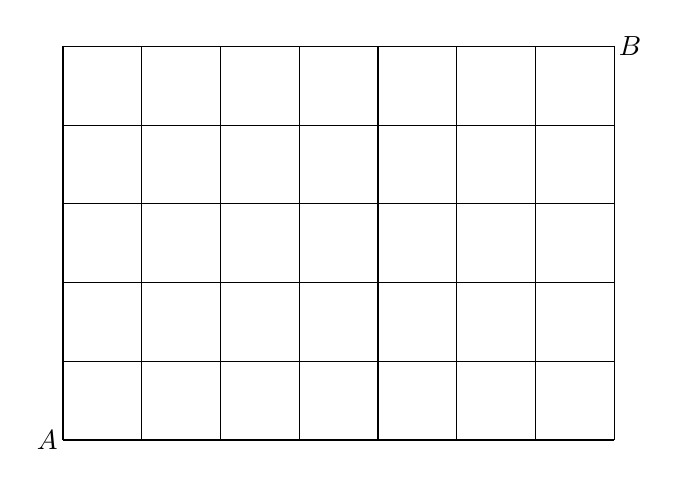
\begin{tikzpicture}
        		\draw (0,0) grid (7,5);
        		\node (a) at (-0.2, 0) {$A$}; 
        		\node (b) at (7.2, 5) {$B$}; 
        \end{tikzpicture}
        \end{center}
		 \end{problem}
		Last time I gave you reasonable grid problems, where you could manually fill out the grid by adding up the number of paths from previous vertices to the next. For this problem, however, the grid seems a little big...
		
		To consider a better way to count the total number of paths, let's just consider a random path that works.
		
		\begin{center}
        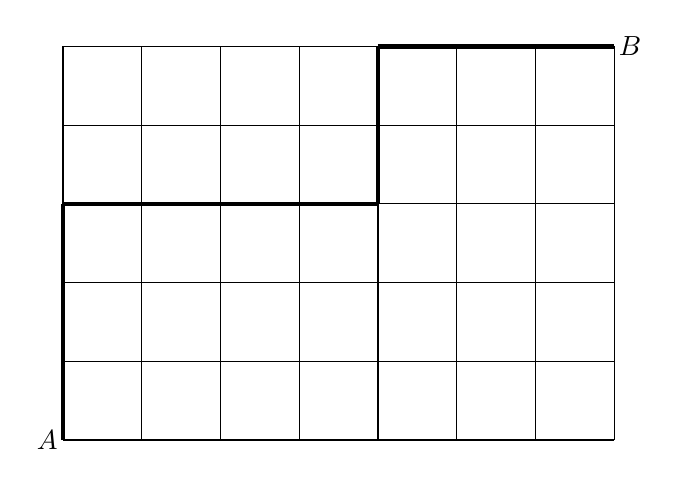
\begin{tikzpicture}
    		\draw (0,0) grid (7,5);
    		\node (a) at (-0.2, 0) {$A$}; 
    		\node (b) at (7.2, 5) {$B$}; 
    		\draw[ultra thick] (0,0) -- (0,3);
    		\draw[ultra thick] (0,3) -- (4,3);
    		\draw[ultra thick] (4,3) -- (4,5);
    		\draw[ultra thick] (4,5) -- (7,5);
        \end{tikzpicture}
        \end{center}
		If we write out the steps to the path above, we get ``UUURRRRUURRR'', where U is ``up'' and R is ``right''. If you play around a bit---in fact, go ahead and draw some paths and write out the steps---you can convince yourself that no matter what your path is, you will end up moving up 5 times and right 7 times. 
		
		Finally, you come to the realization that...``Hey! I just need to count the total number of ways to arrange a word with 5 U's and 7 R's!!!'' And you'd be right, and you'd also be happy to hear you've just derived the formula for finding the number of ways to walk a $m\times n$ grid.
		
		$$\boxed{\text{Number of ways to walk a } m\times n \text{ grid} = \binom{m + n}{n}}$$
		
	\subsection{Paths with Restraints}			
	    Let's begin with a simple problem.

	    \begin{problem}
		 I am currently at home ($A$) and I want to make my way to work at $B$. However, I know there is an accident at point $C$ in the city, so I want to avoid routes that pass through there. Taking this into consideration, how many ways can I drive from $A$ to $B$ if I must not pass through $C$?
		 \begin{center}
        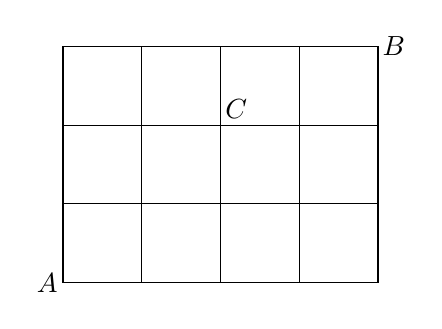
\begin{tikzpicture}
        		\draw (0,0) grid (4,3);
        		\node (a) at (-0.2, 0) {$A$}; 
        		\node (c) at (2.2, 2.2) {$C$};
        		\node (b) at (4.2, 3) {$B$}; 
        \end{tikzpicture}
        \end{center}
		 \end{problem}

		Clearly, it's a lot easier to count the number of paths that go through $C$ rather than the other way around. We can subtract from the total number of paths to get the desired answer for the question.
		
		To solve this problem, all we have to do is break it up into two:
		\begin{enumerate}
		    \item Count the number of ways from $A$ to $C$
		    \item Count the number of ways from $C$ to $B$
		    \item By the fundamental counting principle, the total number of ways will be the product of the two ways above
		\end{enumerate}
        
        So in our case, mirroring the steps above:
        \begin{enumerate}
		    \item Ways from $A$ to $C$: $\binom{4}{2} = 6$
		    \item Ways from $C$ to $B$: $\binom{3}{1} = 3$
		    \item Ways from $A$ to $B$ that go through $C$: $6\times 3 = 18$
		\end{enumerate}
		BUT WAIT, \textbf{WE ARE NOT DONE}!!! The question asked us for the paths that \textbf{don't go through} $C$. So we just subtract from the total:
		$$\binom{7}{3} - 18 = 35-18 = \boxed{17}.$$

    \clearpage
	\subsection{Variations and Disguises}
		Many path counting problems are not just blatantly written out...that would be too easy for you guys and no fun of course. Test writers will often try to hide them to make solving the problem an experience rather than chug and plug. Here we see some typical competition path problems including some infamously difficult ones...
		
		\begin{problem}
		How many ways can I walk from $A$ to $B$ if I am allowed to make two left moves along with the right and up moves I am normally allowed to make?
		\begin{center}
        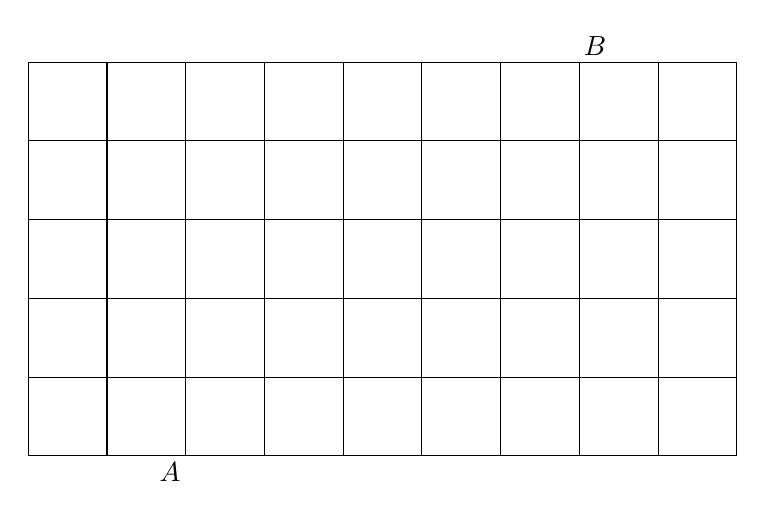
\begin{tikzpicture}
    		\draw (0,0) grid (9,5);
    		\node (a) at (1.8, -0.2) {$A$}; 
    		\node (b) at (7.2, 5.2) {$B$}; 
        \end{tikzpicture}
        \end{center}
        \end{problem}
        
        \begin{problem}
		How many ways can I walk from $A$ to $B$ if I am allowed to make one left move along with the right and up moves I am normally allowed to make? (I am not allowed to walk off the grid!)
		\begin{center}
        \begin{tikzpicture}
    		\draw (0,0) grid (3,2);
    		\node (a) at (-0.2, 0) {$A$}; 
    		\node (b) at (3.2, 2) {$B$}; 
        \end{tikzpicture}
        \end{center}
        \end{problem}
		
		\begin{problem}
		Matt will arrange four identical, dotless dominoes (shaded 1 by 2 rectangles) on the 5 by 4 grid to the right so that a path is formed from the upper left-hand corner A to the lower righthand corner B. In a path, consecutive dominoes must touch at their sides and not just their corners. No domino may be placed diagonally; each domino covers exactly two of the unit squares shown on the grid. One arrangement is shown. How many distinct arrangements are possible, including the one shown? (\textit{Source: MATHCOUNTS State Sprint \#30 2006})
		\begin{center}
        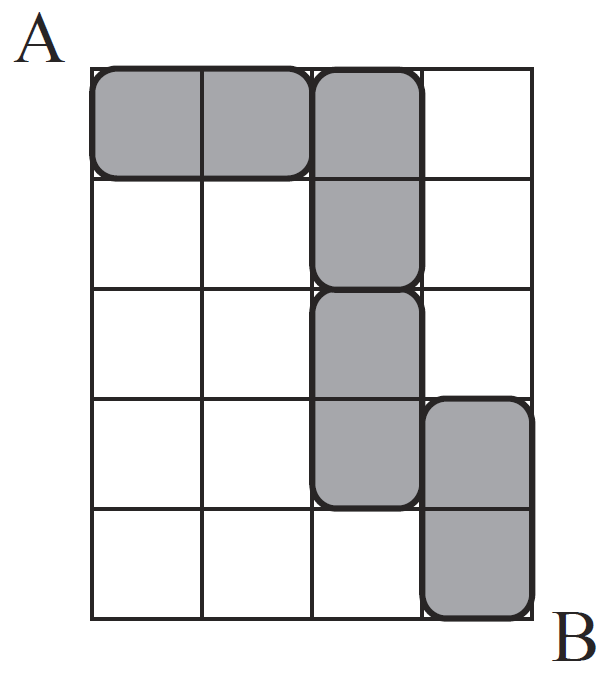
\includegraphics[width=2in]{dominoes}
        \end{center}
		\end{problem}
		
		\clearpage
		
	    \begin{problem}
	    Mack the bug starts at the point (0,0,0) at noon and each minute moves one unit in either the positive $x$-direction, the positive $y$-direction, or the positive $z$-direction. Thus, after 1 minute he could be at (1,0,0), (0,1,0), or (0,0,1). How many different paths could he take to (3,5,2)?
	    \end{problem}

		\begin{problem}
		Cities $A$, $B$, $C$, $D$, and $E$ are connected by roads $\widetilde{AB}$, $\widetilde{AD}$, $\widetilde{AE}$, $\widetilde{BC}$, $\widetilde{BD}$, $\widetilde{CD}$, and $\widetilde{DE}$. How many different routes are there from $A$ to $B$ that use each road exactly once? (Such a route will necessarily visit some cities more than once.)
		\begin{center}
        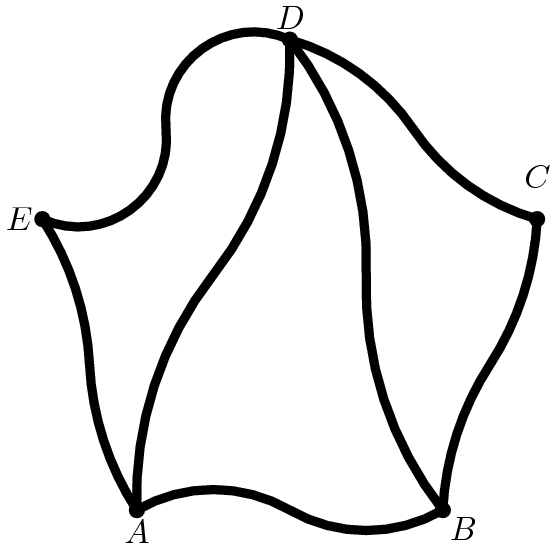
\includegraphics[width=2.5in]{amcgrid}
        \end{center}
		\end{problem}
		
		\begin{problem}
		(\textit{Source: MATHCOUNTS Nationals Sprint \#30})
		\begin{center}
        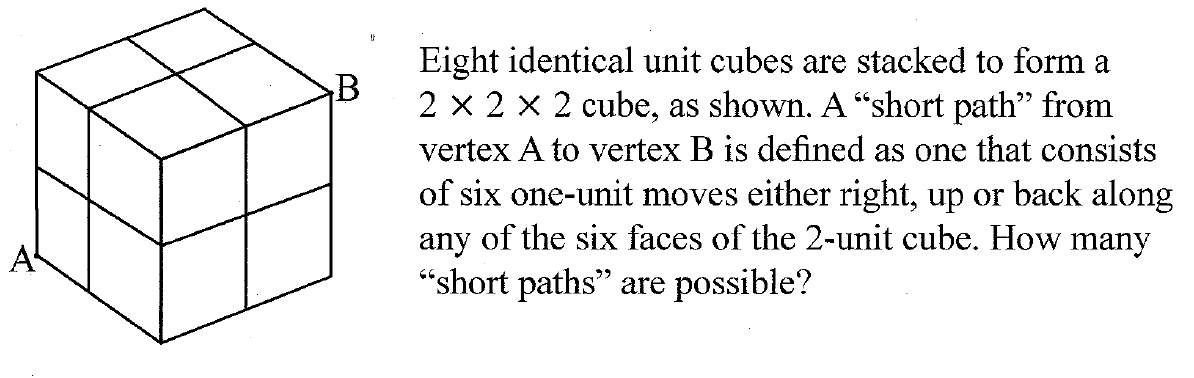
\includegraphics[width=6in]{cube}
        \end{center}
		\end{problem}
		
		\begin{problem}
        In the figure below, how many ways are there to select 5 bricks, one in each row, such that any two bricks in adjacent rows are adjacent? (\textit{HMMT})
        \begin{center}
        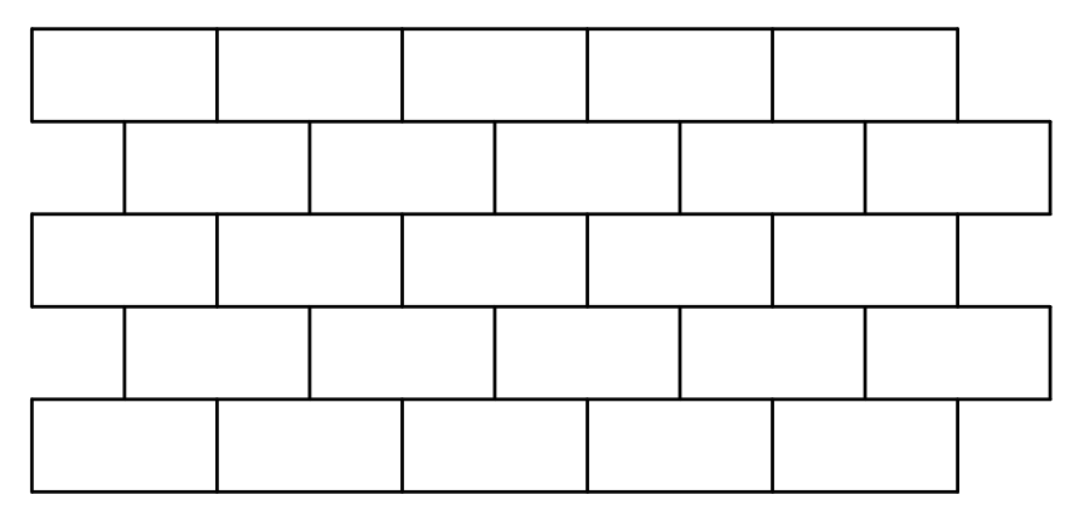
\includegraphics[width=3.5in]{grid}
        \end{center}
        \end{problem}
        
        \clearpage
        
        \begin{problem}
        In the diagram below, how many distinct paths are there from January 1 to December 31, moving from one adjacent dot to the next either to the right, down, or diagonally down to the right? (\textit{HMMT})
        \begin{center}
        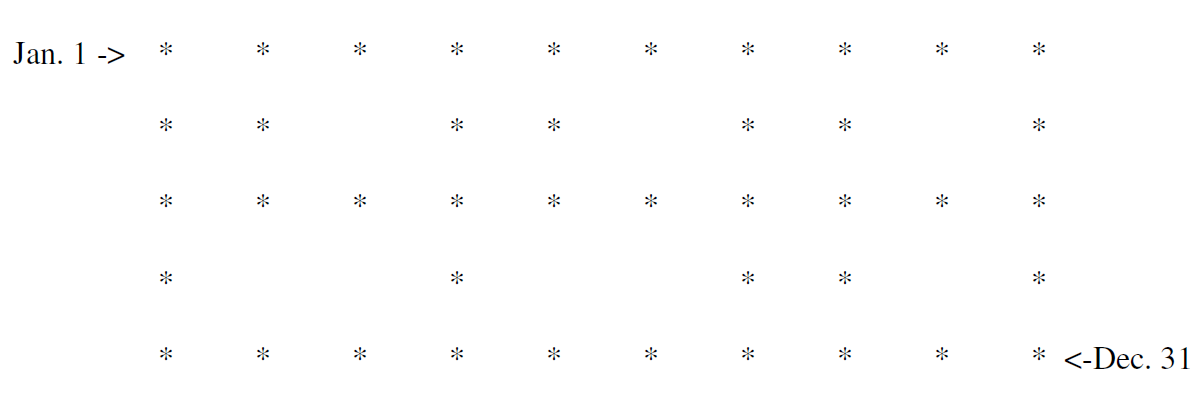
\includegraphics[width=6in]{path2}
        \end{center}
        \end{problem}
		
		\begin{problem}
		A bug travels from A to B along the segments in the hexagonal lattice pictured below. The segments marked with an arrow can be traveled only in the direction of the arrow, and the bug never travels the same segment more than once. How many different paths are there? (\textit{AMC})
        \begin{center}
        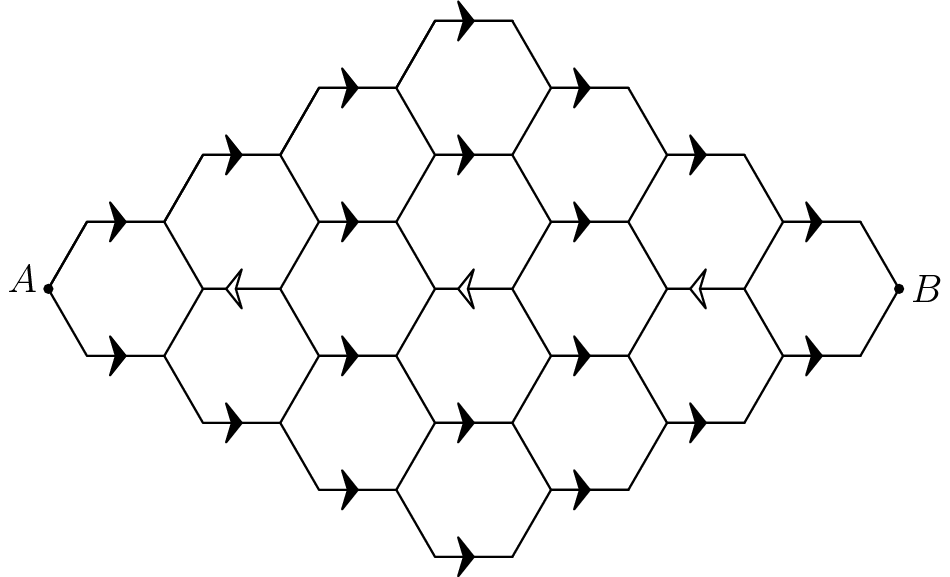
\includegraphics[width=4in]{hexgrid}
        \end{center}
        $\textbf{(A)}\ 2112\qquad\textbf{(B)}\ 2304\qquad\textbf{(C)}\ 2368\qquad\textbf{(D)}\ 2384\qquad\textbf{(E)}\ 2400$
		\end{problem}
		
		\begin{problem}
		I am playing a best-of-three round of rock, paper, scissors with my friend. Since we have played each other a lot, I know the probability that I win any given round is $\frac{2}{3}$, and my friend, $\frac{1}{3}$ (so we never tie). What is the probability I win?
	    \end{problem}
		
		\begin{problem}
		The Patriots and the Seahawks are going to fight a tough game tonight. Due to poor score tracking technology, the two teams can only score with touchdowns (and no extra points), so 6 points whenever a team scores. One analyst predicts the score will be 36-30, with the Patriots winning and never trailing the Seahawks. Another analyst predicts the score will be 42-24, with the Seahawks routing the Patriots, except this time the Seahawks never trail nor tie with the Patriots. How many ways can each of the scenarios happen, and what are their probabilities?
		\end{problem}
		
		\begin{problem}
		The Boston Red Sox and New York Yankees are playing a best of 7 at the World Series. It is well known that for any game, the Yankees have a $\frac{3}{5}$ chance of winning and the Red Sox have a $\frac{2}{5}$ chance of winning. With this knowledge, what is the probability that the teams will go to a game 7?
		\end{problem}